\section{Results}
\label{sec:results}

We organize results by hypothesis. \secref{sec:results-paper} establishes the closed-form decay at the paper layer (H1) and the role of capacity policy as a moderator (H1$'$). \secref{sec:results-researcher} shows the bean-counting failure at the researcher layer (H3). \secref{sec:results-reader} reports the reader-budget consumption analysis (H2). \secref{sec:results-empirical} presents the empirical \iclr calibration (H4) and the model fit.

\subsection{Paper layer: signal decays with volume under fixed capacity}
\label{sec:results-paper}

\Figref{fig:analytical} sweeps the signaling model under fixed capacity $\Kcap{=}200$, Gaussian quality, and reviewer noise $\sigrev \in \{0.3, 0.7, 1.0, 1.5, 2.0\}$. Two qualitative facts are visible immediately. {\bf Mutual information} $\miquant$ peaks near $\Nsub \approx \Kcap/\arate^*$ for some optimum $\arate^*$ and decays monotonically thereafter (Kendall $\tau$ from $-0.51$ at $\sigrev{=}0.3$ to $-0.78$ at $\sigrev{=}1.5$, $p<0.005$ for $\sigrev\le 1.5$). {\bf Tail recall} $\Pr(\acc{=}1\mid \quality \in \text{top-1\%})$ collapses uniformly: Kendall $\tau = -1.0$, $p = 5.5\times 10^{-7}$ for every $\sigrev$, with only $\sim 5\%$ of true top-1\% papers accepted at $\Nsub = 102{,}400$.

\begin{figure}[t]
    \centering
    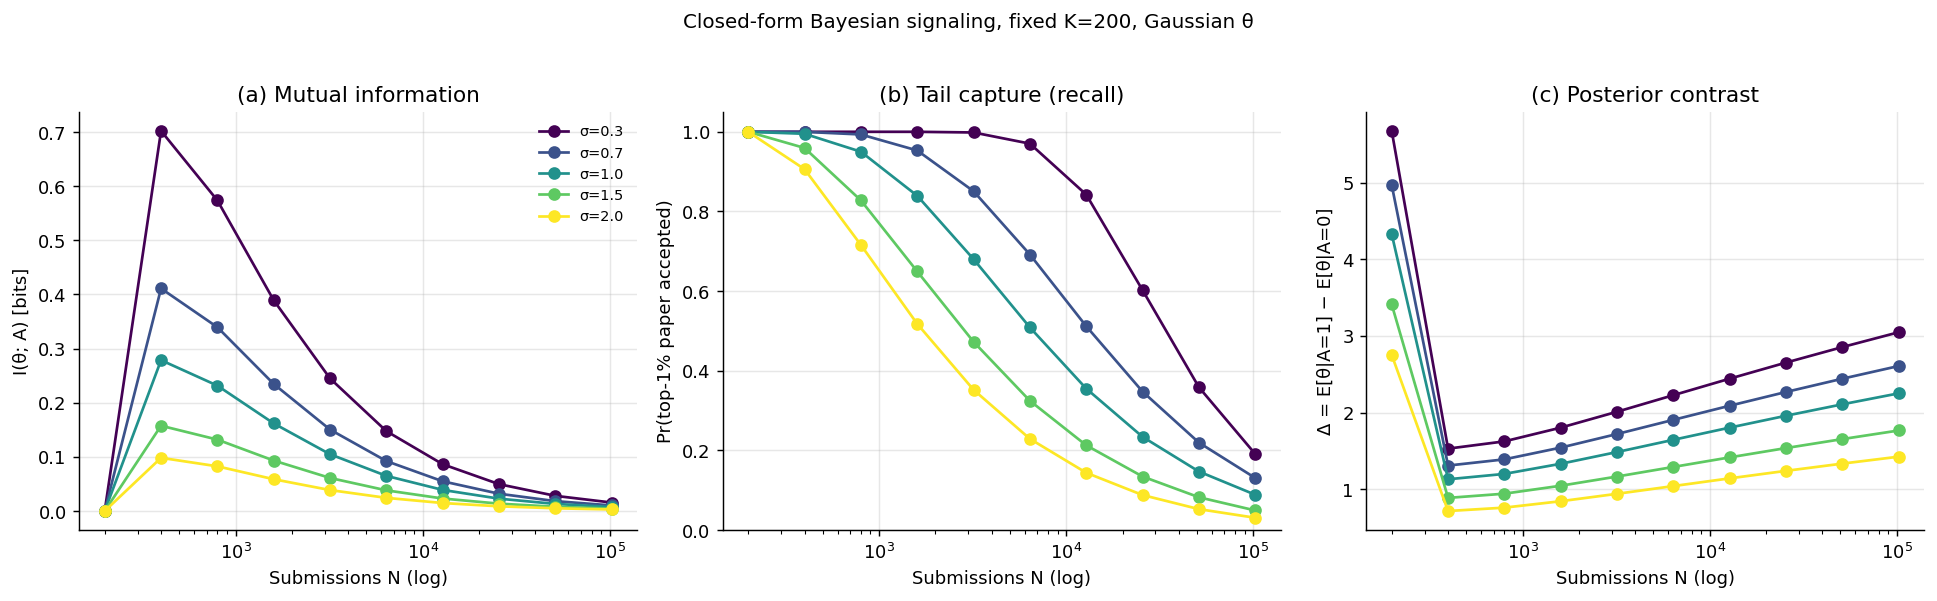
\includegraphics[width=0.95\linewidth]{figures/fig3_analytical_signaling.png}
    \caption{Paper-layer signal decay under fixed capacity $\Kcap{=}200$, Gaussian quality, varying reviewer noise $\sigrev$. \figleft Mutual information $\miquant$ peaks near $\Nsub\sim 1{,}000$ and decays monotonically thereafter. \figcenter Posterior contrast $\contrast = \E[\quality\mid\acc{=}1] - \E[\quality\mid\acc{=}0]$ \emph{increases} in $\Nsub$ because the gatekeeper pulls deeper into the right tail---this masquerades as good news per acceptance but coexists with vanishing recall. \figright Tail recall on the true top-1\% drops to $\sim 5\%$ at $\Nsub{=}102{,}400$ (Kendall $\tau = -1.0$ for every $\sigrev$).}
    \label{fig:analytical}
\end{figure}

The behavior of $\contrast$ deserves comment. A naive operationalization of the hypothesis predicts $\contrast \to 0$. We find the opposite: as $\arate \to 0$, the gatekeeper accepts only the extreme right tail, so the posterior mean $\E[\quality \mid \acc{=}1]$ rises. The information-theoretic quantity $\miquant$ falls anyway because acceptances become rare ($H(\acc) \to 0$ even as the per-acceptance posterior sharpens). {\bf The operationally important quantity that decays is information / recall, not the headline contrast}---a subtlety that the rest of the paper takes seriously.

\para{Robustness across distributions.} \Figref{fig:dist} repeats the sweep with log-normal and Pareto quality. The $\miquant$ peak moves but the decay structure is the same; tail recall drops monotonically in all three.

\begin{figure}[t]
    \centering
    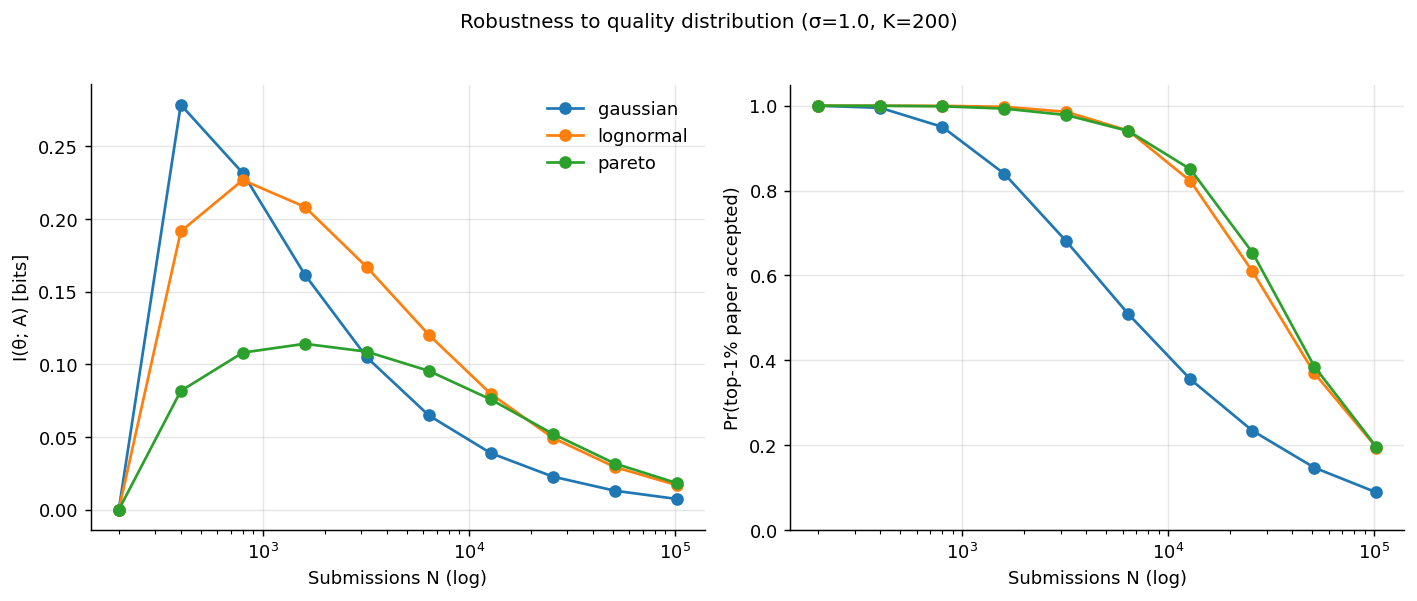
\includegraphics[width=0.95\linewidth]{figures/fig4_distribution_robustness.png}
    \caption{Robustness across quality distributions. The qualitative pattern---peak then decay of $\miquant$, monotone collapse of tail recall---survives the move from Gaussian to log-normal and to Pareto quality. The Pareto right tail mildly slows the decay but does not change the sign of the trend.}
    \label{fig:dist}
\end{figure}

\para{Capacity policy is the central moderator (H1$'$).} \Figref{fig:capacity} repeats the analytical sweep under three capacity policies. Linear capacity ($\Kcap = \arate \cdot \Nsub$) holds $\miquant$ and tail recall flat in $\Nsub$; sublinear $\Kcap \propto \sqrt{\Nsub}$ decays slowly; constant $\Kcap$ decays fastest. The per-paper signal degradation is therefore not inevitable---it is a property of \emph{how capacity scales with volume}, and journals capped at fixed page counts trade per-acceptance precision for catastrophic recall.

\begin{figure}[t]
    \centering
    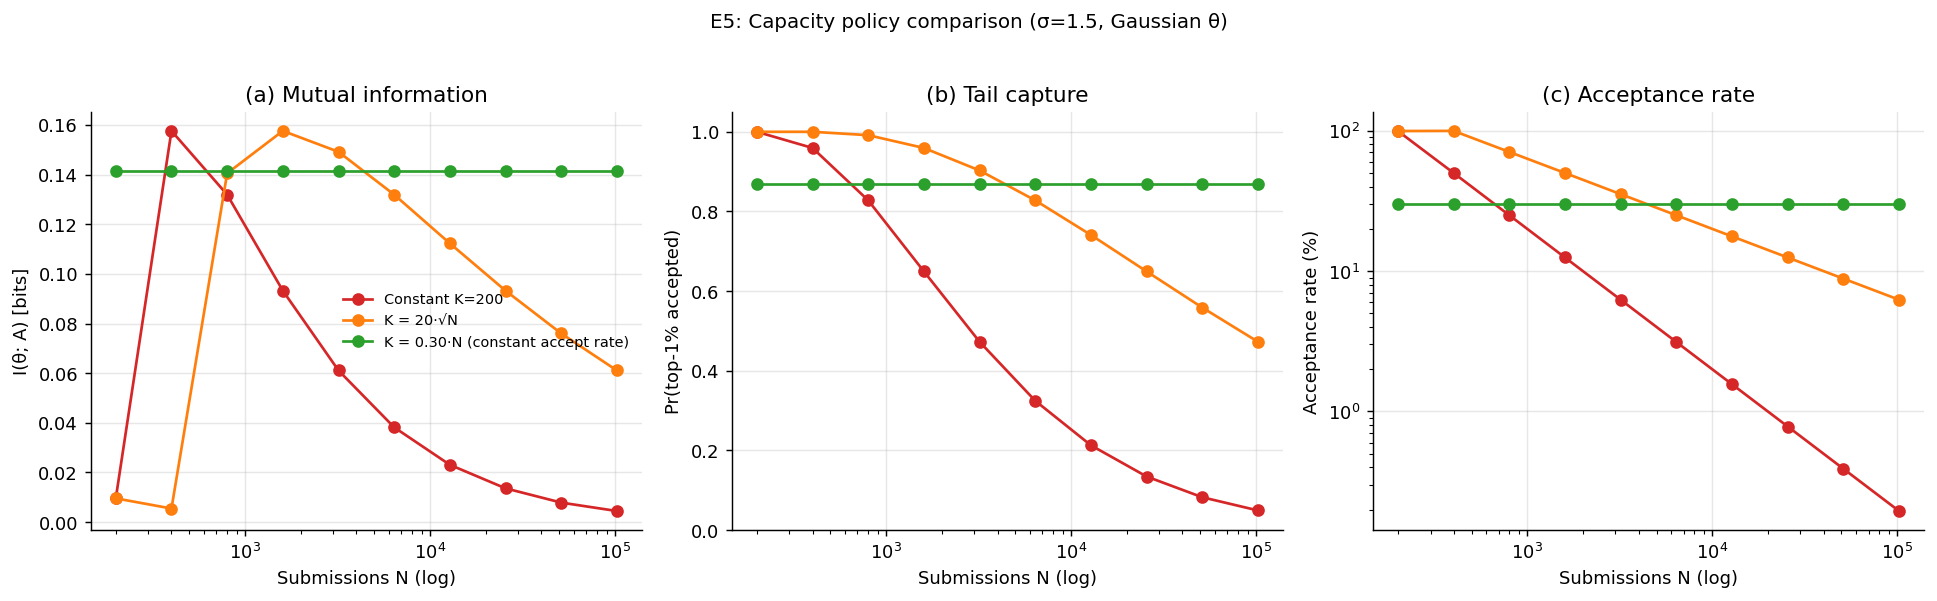
\includegraphics[width=0.95\linewidth]{figures/fig5_capacity_policies.png}
    \caption{Capacity policy as the central moderator. With linear capacity $\Kcap = 0.30\,\Nsub$ (constant accept rate), $\miquant$ and tail recall stay flat in $\Nsub$. Sublinear $\Kcap \propto \sqrt{\Nsub}$ decays slowly. Fixed $\Kcap$ decays fastest. The flat green line recovers the no-capacity-constraint Spence--Akerlof--Long baseline.}
    \label{fig:capacity}
\end{figure}

\subsection{Researcher layer: bean counting fails under fixed capacity}
\label{sec:results-researcher}

\Figref{fig:bean} reports the researcher-level Monte Carlo. \tabref{tab:bean} summarizes the headline numbers. Under {\bf fixed} $\Kcap$, the Spearman correlation between latent ability $\ability$ and publication count $c$ falls monotonically from $0.775 \pm 0.005$ at $M_r{=}200$ to $0.256 \pm 0.003$ at $M_r{=}20{,}000$ (Kendall $\tau = -1.0$, $p = 4\times10^{-4}$; one-sided Mann--Whitney $p = 0.004$ between small- and large-$M_r$ groups). Under {\bf linear} $\Kcap$, the correlation is statistically flat ($p = 0.38$).

\begin{table}[t]
\centering
\caption{Researcher-level identifiability under fixed vs.\ linear capacity. Means $\pm$ SD over $5$ trials. {\bf Bold}: best per row.}
\label{tab:bean}
\begin{tabular}{@{}lccc@{}}
\toprule
Metric & $M_r{=}200$, fixed $\Kcap$ & $M_r{=}20{,}000$, fixed $\Kcap$ & $M_r{=}20{,}000$, linear $\Kcap$ \\
\midrule
Spearman $\rho(\ability, c)$ & $\mathbf{0.775 \pm 0.005}$ & $0.256 \pm 0.003$ & $\mathbf{0.775 \pm 0.002}$ \\
Top-10\% recall & $\mathbf{0.57}$ & $0.28$ & $\mathbf{0.57}$ \\
Researchers with $c{=}0$ (\%) & $\mathbf{2.2}$ & $95.5$ & $12.0$ \\
\bottomrule
\end{tabular}
\end{table}

\begin{figure}[t]
    \centering
    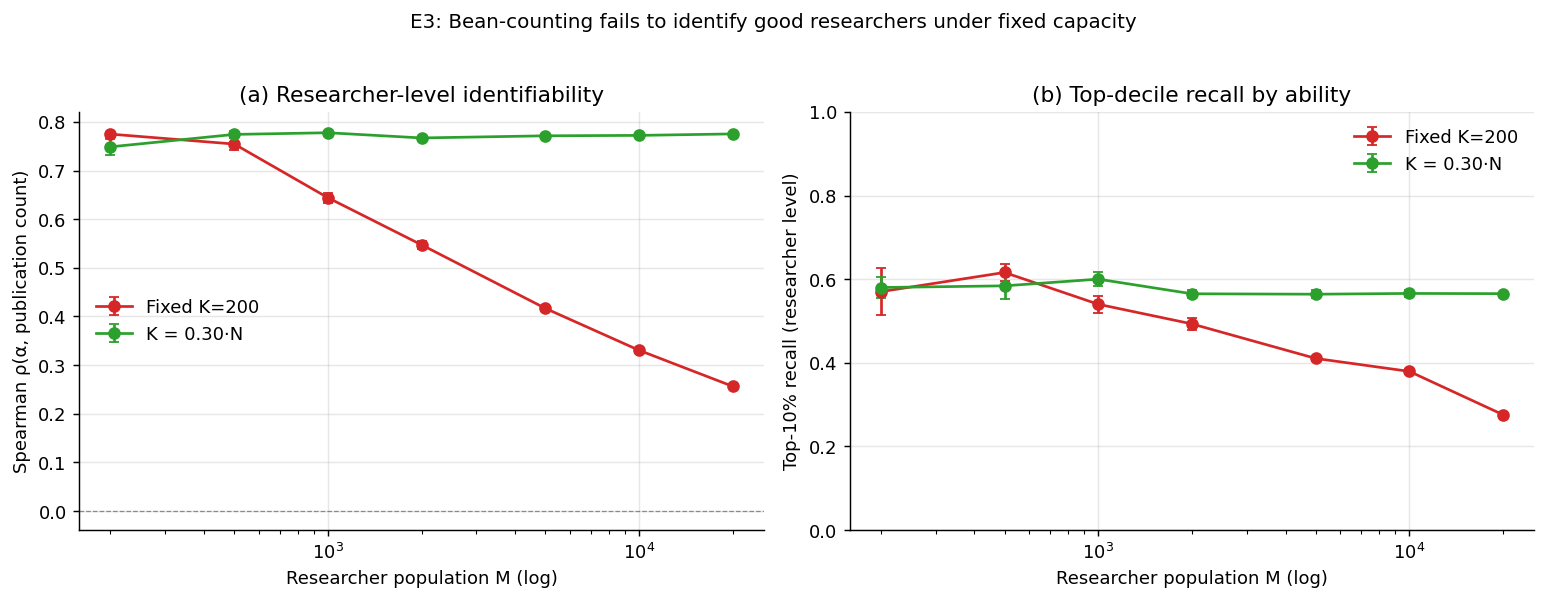
\includegraphics[width=0.95\linewidth]{figures/fig6_bean_counting.png}
    \caption{Researcher-level bean-counting failure. Under fixed capacity, Spearman $\rho(\ability, c)$ falls from $0.78$ at $M_r{=}200$ to $0.26$ at $M_r{=}20{,}000$. The catastrophic mode is mass tying at zero ($95.5\%$ of researchers publish nothing in $T{=}5$ years), so any rank built from publication count is essentially a random tie-break on most of the population. Linear capacity rescues identifiability completely.}
    \label{fig:bean}
\end{figure}

The mechanism behind the collapse is mass tying at zero: $95.5\%$ of researchers publish nothing in $T{=}5$ years under fixed capacity at $M_r{=}20{,}000$, so the rank built from publication count is dominated by tie-breaks on uninformative zero counts. {\bf This formalizes the intuition that publication-count metrics ``reduce to bean counting and bean counting does not surface actually good researchers'' once the field outgrows the venue.}

\subsection{Reader layer: necessary but not sufficient}
\label{sec:results-reader}

\Figref{fig:reader} reports total true quality consumed over $T{=}12$ years for $M{=}200$ readers, $\budget{=}20$ papers/year, $\sigrev{=}1.5$. Under fixed capacity, the gap between sampling from accepted papers and sampling at random {\bf grows} in $\log \Nsub$ (slope $+69.4$ quality units per $e$-fold of $\Nsub$, $p = 1.0\times10^{-5}$). Under linear capacity, the gap is statistically flat at $\sim 155$ quality units (slope $+2.6$, $p = 0.13$).

\begin{table}[t]
\centering
\caption{Reader consumption (total quality over $12$ years $\times \budget{=}20$ papers/year). Means $\pm$ SD over readers.}
\label{tab:reader}
\begin{tabular}{@{}llc@{}}
\toprule
Capacity policy & Sampling strategy & Total quality consumed \\
\midrule
Fixed $\Kcap{=}200$, $\Nsub{=}25{,}600$ & accepted pool & $\mathbf{368.7 \pm 1.0}$ \\
                                          & all submissions & $0.21 \pm 1.13$ \\
\midrule
Linear $\Kcap = 0.30\Nsub$, $\Nsub{=}25{,}600$ & accepted pool & $154.0 \pm 1.0$ \\
                                                  & all submissions & $-0.66 \pm 1.17$ \\
\bottomrule
\end{tabular}
\end{table}

\begin{figure}[t]
    \centering
    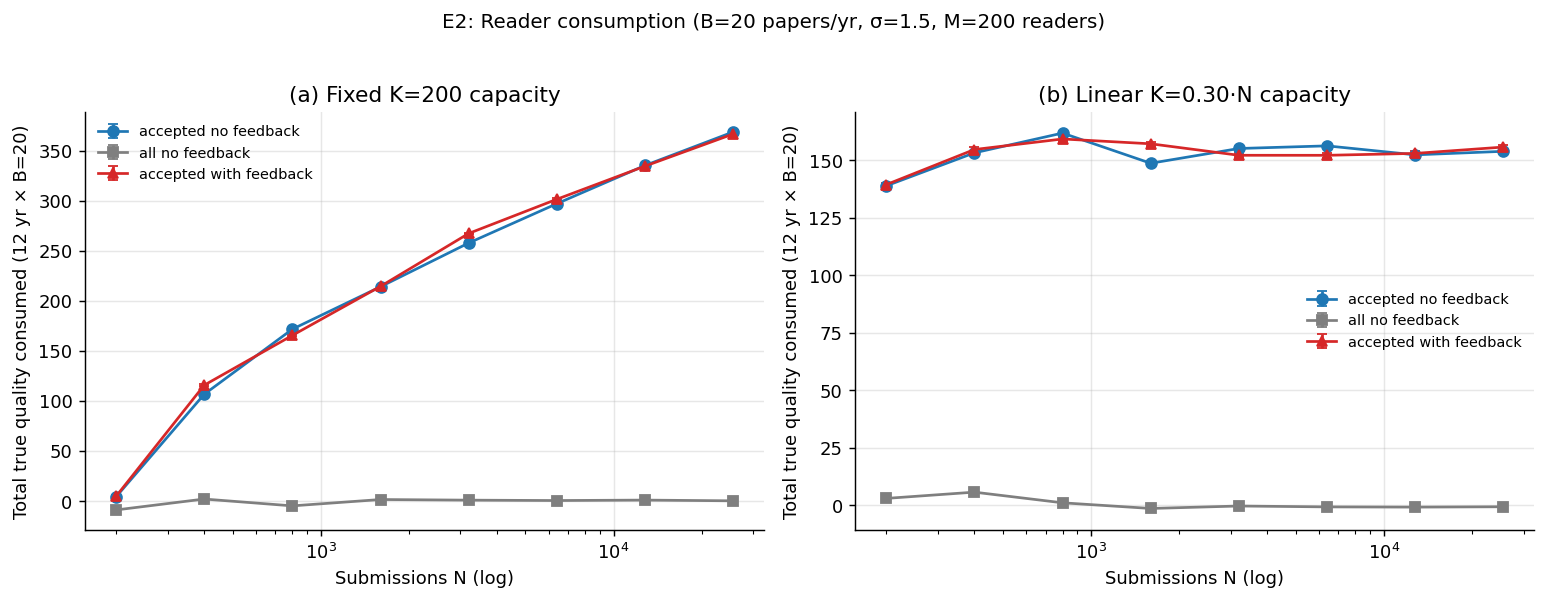
\includegraphics[width=0.95\linewidth]{figures/fig7_consumption.png}
    \caption{Reader-side consumption. Fixed capacity makes the venue label increasingly informative \emph{per accepted paper} (the gap grows in $\log \Nsub$), but with vanishing accepted pool it becomes a Pyrrhic victory. Linear capacity keeps the gap flat in $\Nsub$, but as $\budget/\Kcap \to 0$ the reader can only sample a vanishing fraction of accepted papers---the label tells them to read accepted ones, but cannot tell them which.}
    \label{fig:reader}
\end{figure}

The two regimes produce qualitatively different reader experiences. Under fixed $\Kcap$, the venue label is exquisitely informative per acceptance but identifies a vanishingly small pool. Under linear $\Kcap$, the label survives as a coarse filter but cannot select what to read among thousands of accepted papers---{\bf the venue label remains necessary but ceases to be sufficient}. The negative-experience feedback rule did not trigger reader collapse with our conservative threshold ($\tau_{\text{bad}} = -0.3$), since the average accepted paper has positive quality under both regimes; we revisit this in \secref{sec:discussion}.

\subsection{Empirical calibration on \iclr (H4)}
\label{sec:results-empirical}

\Figref{fig:emp-growth} shows \iclr submission volume from $2013$ ($67$ submissions) to $2026$ ($19{,}814$), a $296\times$ increase. Acceptance rates have stayed near $25$--$35\%$ across all measured years; the venue is operating at constant accept rate, the linear-$\Kcap$ regime in our taxonomy. \Figref{fig:emp-disp} shows that the mean per-paper reviewer SD has grown from $0.86$ in $2017$ to $1.53$ in $2026$ (Kendall $\tau = +0.64$ on year, $p = 0.031$).

\begin{figure}[t]
    \centering
    \begin{subfigure}[b]{0.48\linewidth}
        \centering
        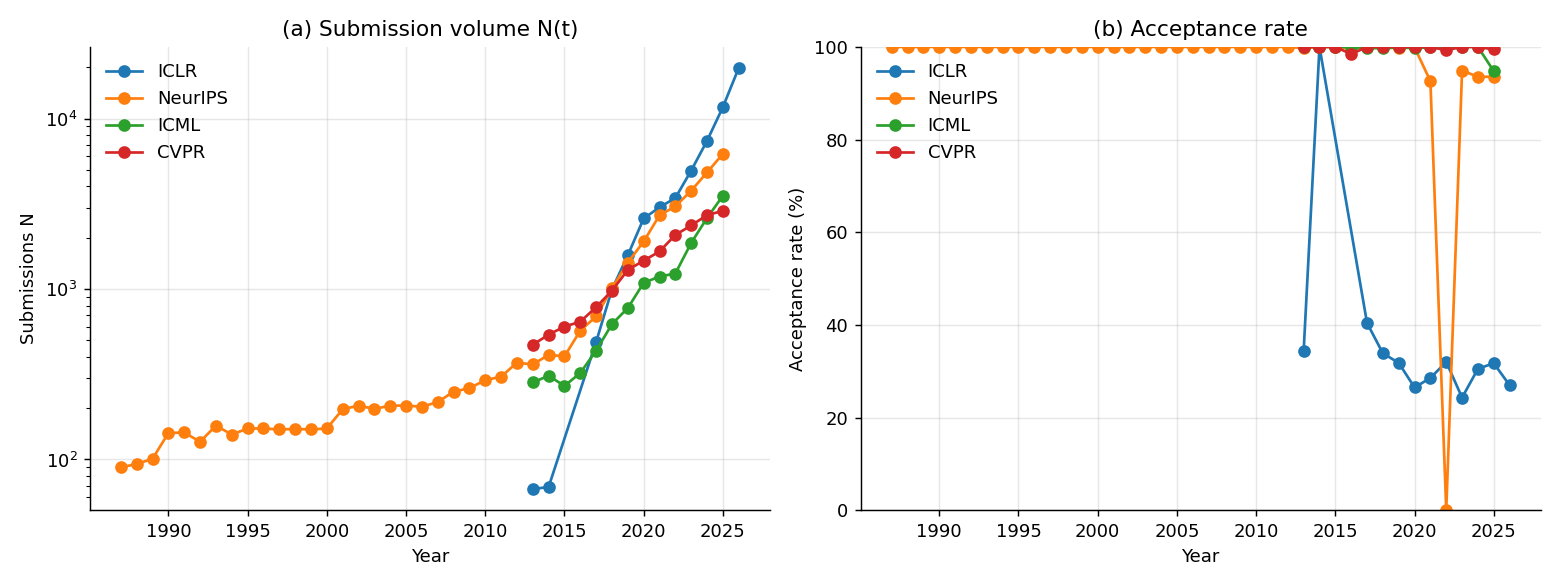
\includegraphics[width=\linewidth]{figures/fig1_empirical_growth.png}
        \caption{\iclr submission volume, $2013$--$2026$.}
        \label{fig:emp-growth}
    \end{subfigure}
    \hfill
    \begin{subfigure}[b]{0.48\linewidth}
        \centering
        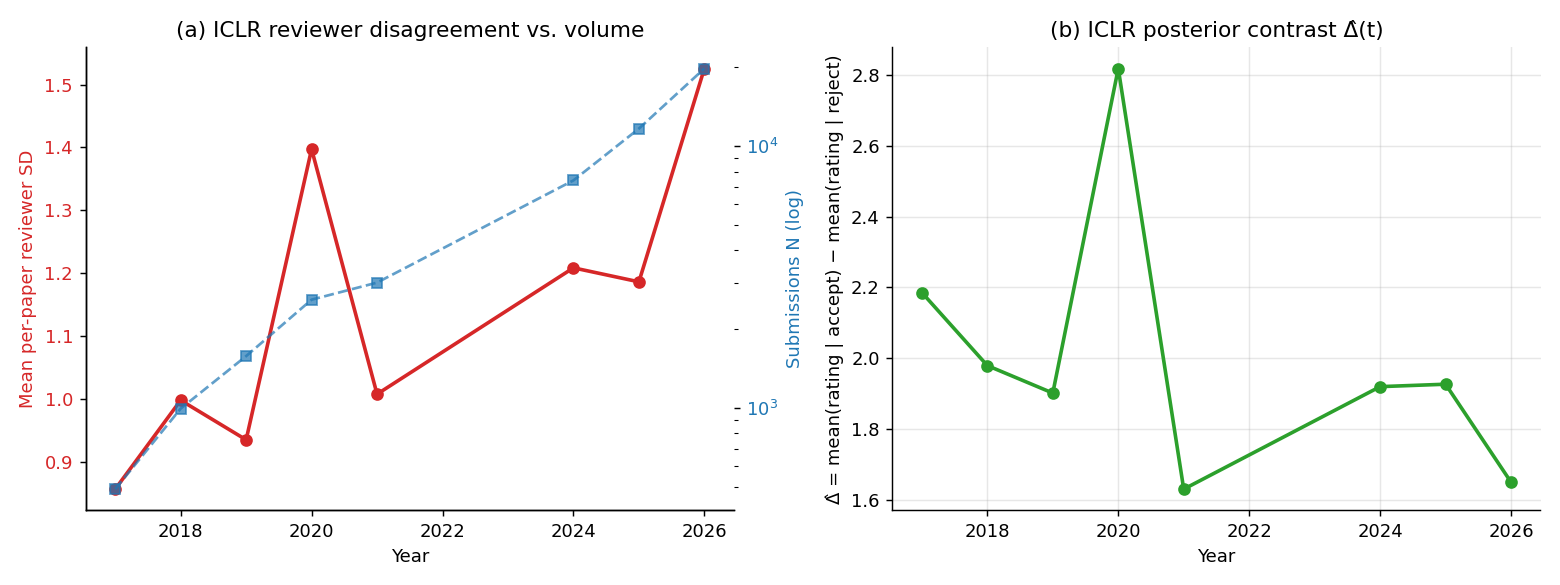
\includegraphics[width=\linewidth]{figures/fig2_empirical_dispersion.png}
        \caption{Mean per-paper reviewer SD over time.}
        \label{fig:emp-disp}
    \end{subfigure}
    \caption{Empirical \iclr trends. \captiona Submissions grew from $67$ in $2013$ to $19{,}814$ in $2026$, a $296\times$ increase; acceptance rate has stayed at $25$--$35\%$, putting \iclr in the linear-$\Kcap$ regime. \captionb Mean per-paper reviewer SD has grown $0.86 \to 1.53$ (Kendall $\tau = +0.64$, $p = 0.031$), consistent with load-induced noise.}
    \label{fig:emp}
\end{figure}

\Tabref{tab:iclr} compiles the standardized posterior contrast $\hcontrast / \stdrating$ across years. The headline empirical result: an OLS regression of $\hcontrast / \stdrating$ on $\log \Nsub$ has slope $-0.318$, $p = 1.14\times10^{-3}$, $R^2 = 0.85$. {\bf Per $e$-fold growth in $\Nsub$, the standardized signaling contrast falls by $0.32$ SD units}, from $2.55$ at $\Nsub{=}490$ to $1.08$ at $\Nsub{=}19{,}814$.

\begin{table}[t]
\centering
\caption{\iclr standardized signaling contrast vs.\ year. $\hcontrast = \E[\bar r\mid\acc{=}1] - \E[\bar r\mid\acc{=}0]$; $\stdrating$ is the rating SD. Standardized contrast falls $58\%$ as $\Nsub$ grows $40\times$.}
\label{tab:iclr}
\begin{tabular}{@{}lcccc@{}}
\toprule
Year & $\Nsub$ & Mean reviewer SD & $\hcontrast$ (raw) & $\hcontrast / \stdrating$ \\
\midrule
$2017$ & $490$ & $0.86$ & $2.19$ & $\mathbf{2.55}$ \\
$2020$ & $2{,}594$ & $1.40$ & $2.82$ & $2.02$ \\
$2024$ & $7{,}407$ & $1.21$ & $1.92$ & $1.59$ \\
$2026$ & $19{,}814$ & $1.53$ & $1.65$ & $\mathbf{1.08}$ \\
\bottomrule
\end{tabular}
\end{table}

\para{Model calibration.} \Figref{fig:calib} fixes the model's capacity policy to \iclr's actual yearly acceptance rate and searches for the reviewer noise $\sigrev$ that best matches $\hcontrast / \stdrating$. The inferred $\sigrev$ rises from $0.5$ (2017--2025) to $1.0$ (2026), tracking the rise in measured per-paper reviewer SD ($0.86 \to 1.53$). This is the {\bf load-induced noise mechanism} in action: \iclr expanded capacity linearly with $\Nsub$, so the linear-$\Kcap$ row of \secref{sec:results-paper} predicts that per-paper precision should hold \emph{if} reviewer noise stayed constant. The signal degraded anyway, and the same expansion that preserved per-paper precision under the analytical model is exactly what forces $\sigrev$ to grow because the reviewer pool did not expand commensurately.

\begin{figure}[t]
    \centering
    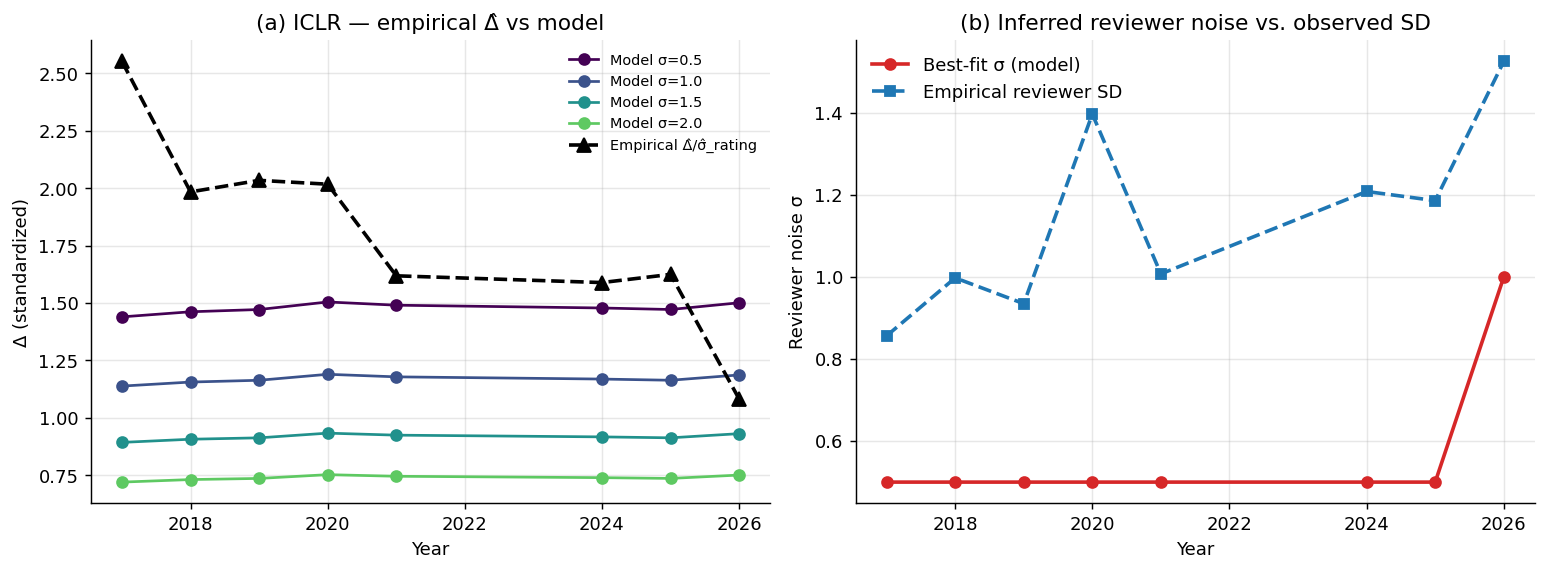
\includegraphics[width=0.7\linewidth]{figures/fig8_calibration_iclr.png}
    \caption{Model calibration to \iclr. With \iclr's empirical accept rate as the capacity policy, the reviewer noise $\sigrev$ that minimizes RMSE on $\hcontrast / \stdrating$ rises from $\sim 0.5$ to $\sim 1.0$ between $2017$ and $2026$. This is precisely the load-induced-noise channel: linear capacity expansion preserves the analytical signal, but only if the reviewer pool expands too, which it has not.}
    \label{fig:calib}
\end{figure}

\para{Comparison to baselines.} The flat green line in \figref{fig:capacity} reproduces the no-capacity-constraint Spence--Akerlof--Long invariance. The tail-recall metric in moderate-$\Nsub$/moderate-$\sigrev$ cells reproduces \citet{heckman2019tyranny}'s $\sim 50\%$ top-paper capture by the top tier. Our calibrated $\sigrev = 1.0$ for \iclr 2026 is in the same range as the Cortes--Lawrence $\sim 50\%$ disagreement noise floor.
